% !TEX root = ../paper.tex

\section{Experimental Results}
\label{sec:results}

\subsection{Experimental Platform}
\label{sec:summit}

All the experiments in this section were conducted on Summit. Summit is a supercomputer created by IBM for the Oak Ridge National Laboratory. 
There are approximately 4,600 nodes on Summit. 
Each node contains two IBM POWER9 processors on separate sockets with 512 GB of DDR4 memory.
Each POWER9 processor utilizes 22 IBM SIMD Multi-Cores (SMCs), although one of these SMCs on each processor is dedicated to memory transfer and is therefore not available for computation. 
For node scaling experiments, all 42 available SMCs were utilized in each node so that every node computed with 42 separate MPI processes.
Additionally, every node also supports six NVIDIA Volta V100 accelerators but these were unused by our algorithm. 

Our implementation builds on the PLANC open-source library \cite{EH+19-TR} and uses the Armadillo library (version 9.900.1) for all matrix operations. 
On Summit, we linked this version of Armadillo with OpenBLAS (version 0.3.9) and IBM's Spectrum MPI (version 10.3.1.2-20200121).

\subsection{Datasets}

\paragraph{\emph{Hyperspectral Imaging}}

	We use the Hyperspectral Digital Imagery Collection Experiment (HYDICE) image of the Washington DC Mall. We will refer
	to this dataset as \hyper{}\cite{DC-HYDICE}.
	
	\hyper{} is formatted into a 3-way tensor representing two spatial dimensions of pixels and one dimension of spectral bands. So, a slice along
	the spectral band dimension would be the full \hyper{} image in that spectral band. For hierarchical clustering, these tensors are flattened so that the rows represent the
	$191$ spectral bands and the columns represent the $392960$ pixels.   The data set is approximately 600 MB in size.

	%Larger hyperspectral datasets tend to not grow larger than around 200 spectral bands and have millions or billions of pixels. So, scaling is 
	%limited for this dataset given our data distribution scheme.
	
\paragraph{\emph{Image Classification}}

	The SIIM-ISIC Melanoma classification
	dataset, which we will refer to as \image{}\cite{SIIM-ISIC}, consists of $33126$ RGB training images equally sized at $1024 \times 1024$. Unlike with hyperspectral imaging, the resulting
	matrix used in hierarchical clustering consists of image pixels along the rows and individual images along the columns. So, the resulting sized matrix is
	$3145728 \times 33126$, which is approximately 800 GB in size. 

	Given its size, \image{} requries $10$ Summit nodes to perform hierarchical clustering.
	
\paragraph{\emph{Synthetic Dataset}}

	Our synthetic dataset has the same aspect ratio of \image{} but consists of fewer rows and columns by a factor of $3$. The resulting matrix is $1048576 \times 11042$. 
	We choose the smaller size in order to fit on a single node for scaling experiments.

\subsection{Performance}
\label{sec:perf}
For all hierarchical clustering experiments in this section, the number of tree leaf nodes $k$ was set at $100$, 
the number of NMF iterations was set to $100$,
the power iteration was allowed to stop iterating after convergence,
and only complete levels were considered for analysis purposes for both level and strong scaling plots.

\subsubsection{Single-Node Scaling for DC Dataset}

\hyper{} is small compared to the other datasets, so it can easily fit on one compute node.
Also, its small number of 191 rows doesn't allow for parallelizing beyond that number of MPI processes.
So, this dataset was used for a single-node scaling experiment on Summit from 1 to 42 cores.
Because Rank-2 NMF is memory bandwidth bound, we expect limited speedup on one node due to the memory bandwidth not scaling linearly with the number of cores. 
\Cref{fig:dcspeedup} shows that there is enough speedup (14$\times$ on 42 cores) for it to be worth parallelizing such a small problem, but perfect scaling requires more memory bandwidth. 
In this experiment, the processes were distributed across both sockets so that an even number of cores on each socket are used.

\begin{figure}
\begin{center}
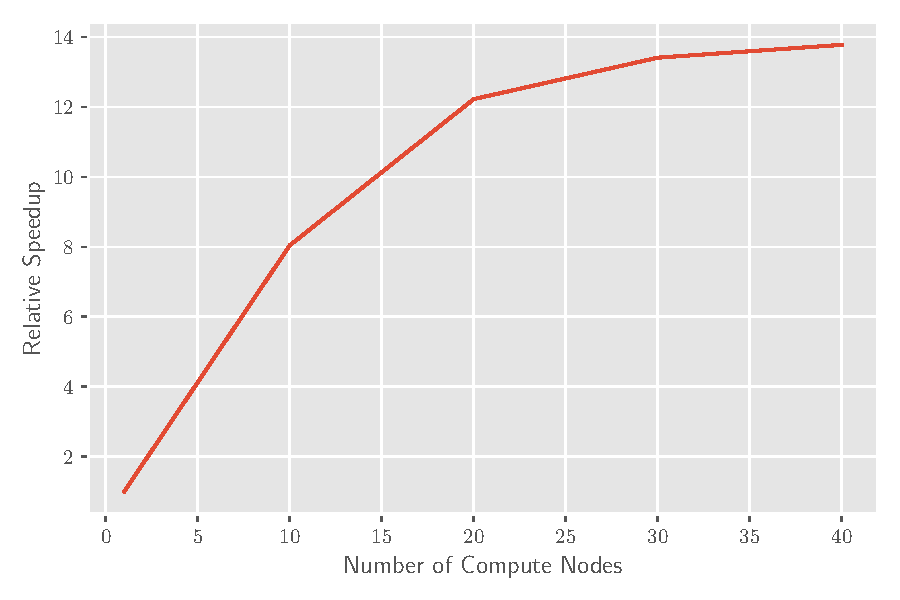
\includegraphics[height=2in, width=\columnwidth]{plots/dc_hierarchical_speedup.pdf}
\caption{Strong Scaling Speedup for Hierarchical Clustering on \hyper{}}
\label{fig:dcspeedup}
\end{center}
\end{figure}


\subsubsection{Rank-2 NMF Strong Scaling}

We perform strong scaling experiments for a single Rank-2 NMF (\Cref{alg:parrank2nmf}) on the synthetic and \image{} datasets.
The theory (\Cref{eq:r2nmfcost}) suggests that perfect strong scaling is possible as long as the execution time is dominated by local computation.
Both the matrix multiplications and NNLS solves scale linearly with $1/p$ (we expect MatMul to dominate), but the bandwidth cost is independent of $p$ and the latency cost increases slightly with $p$.

\Cref{fig:synrank2speedup,fig:rwrank2speedup} show performance relative to the smallest number of compute nodes required to store data and factor matrices.
For these data sets, we observe nearly perfect strong scaling, with 42$\times$ speedup on 40 compute nodes (over 1 compute node) for synthetic data and 7.1$\times$ speedup on 80 compute nodes (over 10 compute nodes) for \image{} data.

\begin{figure}
\begin{center}
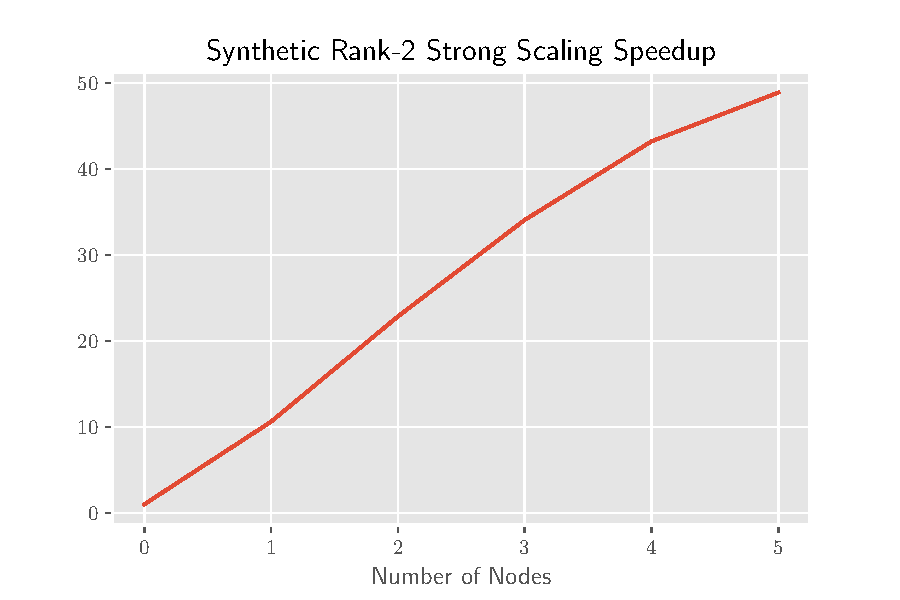
\includegraphics[height=2in, width=\columnwidth]{plots/synthetic_rank2_speedup.pdf}
\caption{Strong Scaling Speedup for Rank-2 NMF on Synthetic Data}
\label{fig:synrank2speedup}
\end{center}
\end{figure}

\begin{figure}
\begin{center}
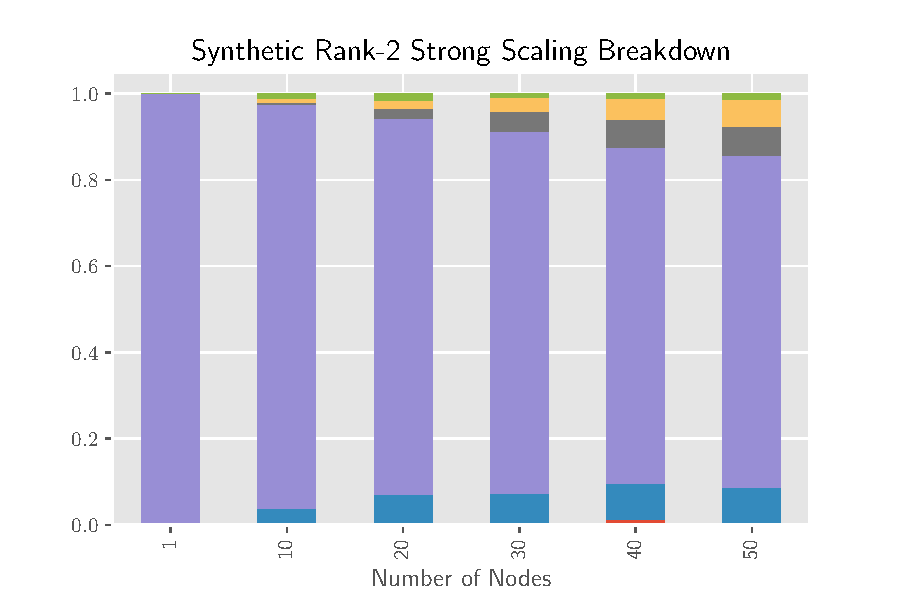
\includegraphics[height=2in, width=\columnwidth]{plots/synthetic_rank2_strongscaling.pdf}
\caption{Relative Time Breakdown for Rank-2 NMF on Synthetic Data}
\label{fig:synrank2strongscaling}
\end{center}
\end{figure}

The relative time breakdowns are presented in \Cref{fig:synrank2strongscaling,fig:rwrank2strongscaling} and explain the strong scaling performance.
Each experiment is normalized to 100\% time, so comparisons cannot be readily made across numbers of compute nodes. 
For both data sets, we see that the time is dominated by MatMul, which is the primary reason for the scalability.
The dominant matrix multiplications are between a large matrix and a matrix with 2 columns, so it is locally memory bandwidth bound, with performance proportional to the size of the large matrix.
In each plot, we also see the relative time of all-gather and reduce-scatter increasing, which is because the local computation is decreasing while the communication cost is slightly increasing with $p$.
This pattern will continue as $p$ increases, which will eventually limit scalability, but for these data sets the MatMul takes around 80\% of the time at over 2000 cores.

\begin{figure}
\begin{center}
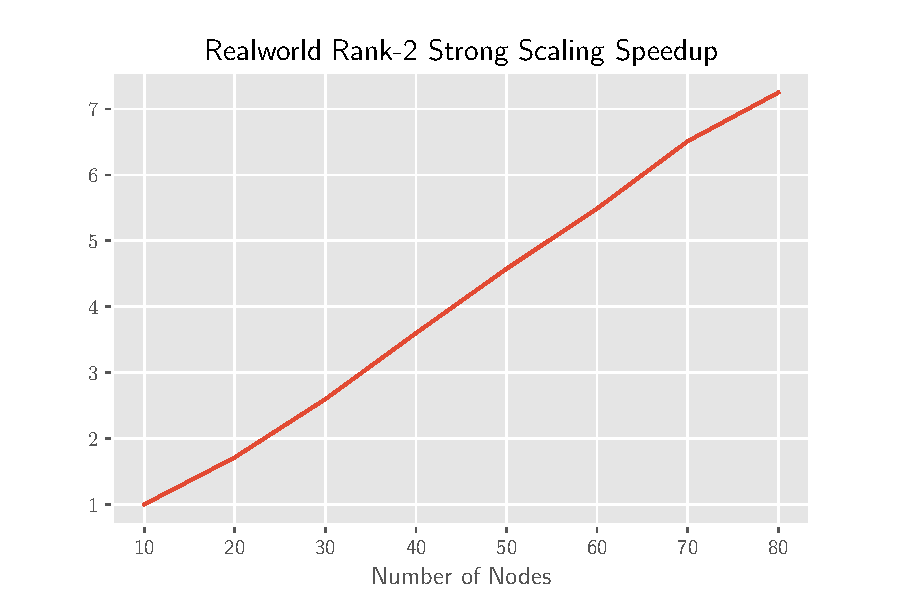
\includegraphics[height=2in, width=\columnwidth]{plots/realworld_rank2_speedup.pdf}
\caption{Strong Scaling Speedup for Rank-2 NMF on \image{} Data}
\label{fig:rwrank2speedup}
\end{center}
\end{figure}

\begin{figure}
\begin{center}
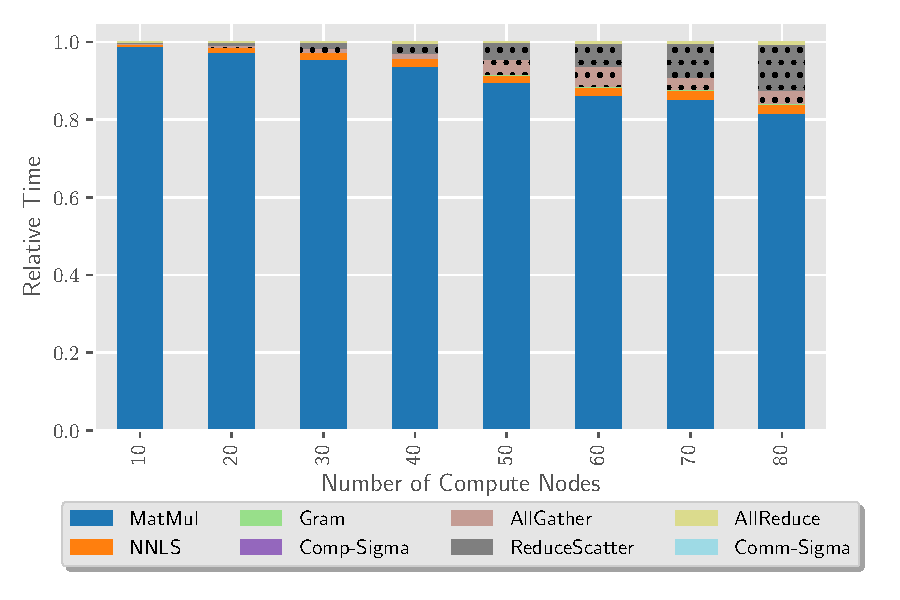
\includegraphics[height=2in, width=\columnwidth]{plots/realworld_rank2_strongscaling.pdf}
\caption{Relative Time Breakdown for Rank-2 NMF on \image{} Data}
\label{fig:rwrank2strongscaling}
\end{center}
\end{figure}


\subsubsection{Hierarchical Clustering Strong Scaling}
\label{sec:hiernmf2scaling}

From \Cref{eq:treecost}, we expect to see perfect strong scaling in a computationally bound hierarchical clustering problem with target cluster count $k=100$.
As $k$ is large, we expect the latency cost of small problems deep in the tree to limit scalability.

\Cref{fig:synhierspeedup} demonstrates the scalability of the synthetic data set on up to 40 nodes, and we observe a 15$\times$ speedup compared to 1 node.
\Cref{fig:synhierstrongscaling} shows the relative time breakdown and explains the limitation on scaling.
On 40 nodes, computation still takes 60\% of the total time, but the all-gather and reduce-scatter costs have grown in relative time because they do not scale with $p$.
Because all-reduce involves only a constant amount of data and its time remains relatively small, we conclude the communication is bandwidth bound at this scale.

With the larger \image{} dataset, it's possible to scale much further as seen in \Cref{fig:rwhierspeedup}, where we observe a 5.9$\times$ speedup of 80 compute nodes compared to 10.
From \Cref{fig:rwhierstrongscaling}, we see that the communication cost constitutes less than 20\% of the total time even at 80 compute nodes. 

We note that the speedup of the overall hierarchical clustering algorithm is not as high as for a single Rank-2 NMF (measured at the root node).
This is due to inefficiencies in the lower levels of the tree, as we explore in the next section.

\begin{figure}
\begin{center}
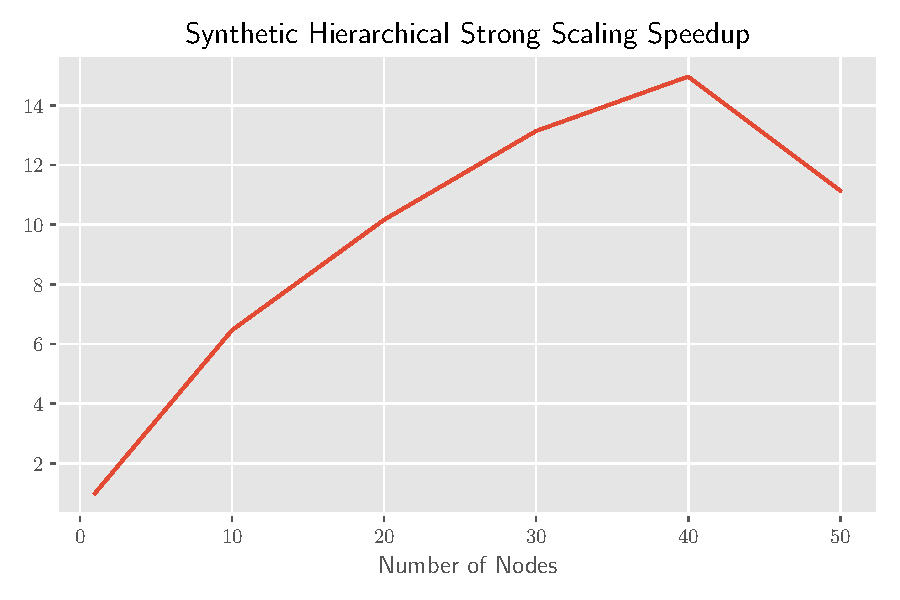
\includegraphics[height=2in, width=\columnwidth]{plots/synthetic_hierarchical_speedup.pdf}
\caption{Strong Scaling Speedup for Hierarchical Clustering on Synthetic Data}
\label{fig:synhierspeedup}
\end{center}
\end{figure}

\begin{figure}
\begin{center}
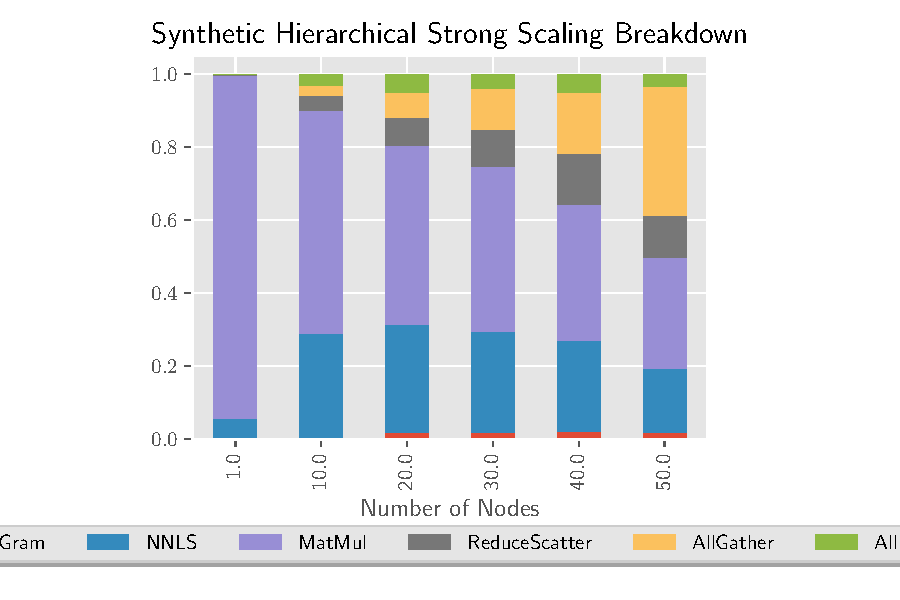
\includegraphics[height=2in, width=\columnwidth]{plots/synthetic_hier_strongscaling.pdf}
\caption{Relative Time Breakdown for Hierarchical Clustering on Synthetic Data}
\label{fig:synhierstrongscaling}
\end{center}
\end{figure}

\begin{figure}
\begin{center}
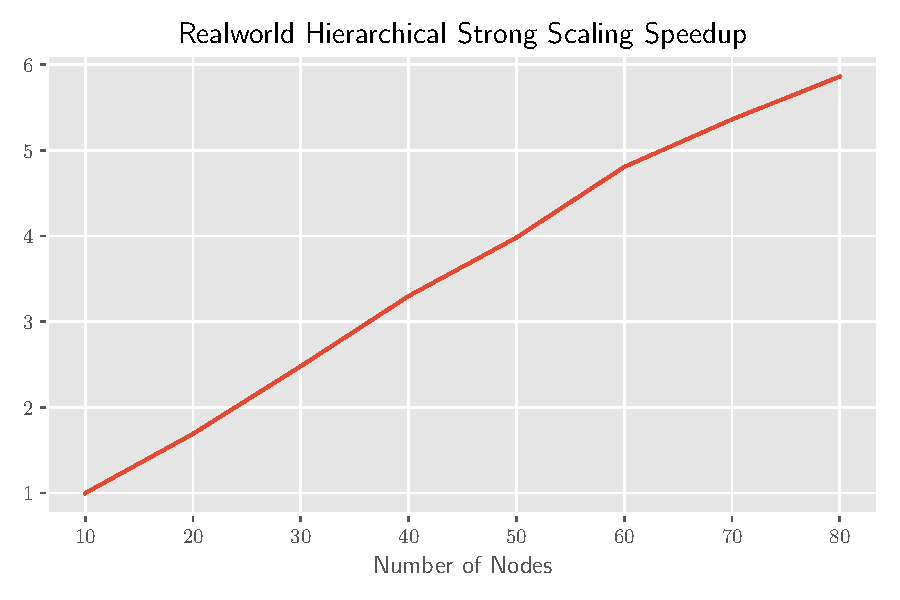
\includegraphics[height=2in, width=\columnwidth]{plots/realworld_hierarchical_speedup.pdf}
\caption{Strong Scaling Speedup for Hierarchical Clustering on \image{} Data}
\label{fig:rwhierspeedup}
\end{center}
\end{figure}

\begin{figure}
\begin{center}
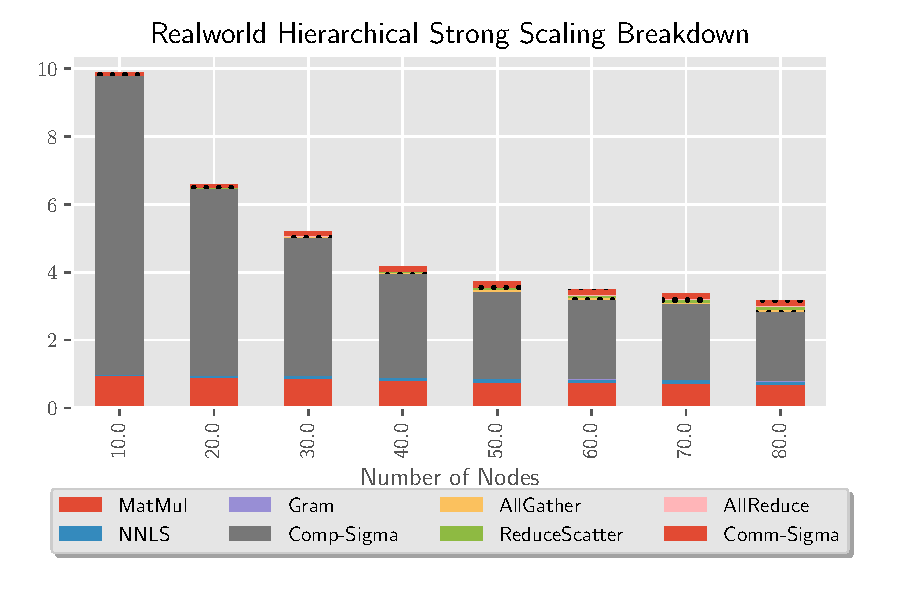
\includegraphics[height=2in, width=\columnwidth]{plots/realworld_hier_strongscaling.pdf}
\caption{Relative Time Breakdown for Hierarchical Clustering on \image{} Data}
\label{fig:rwhierstrongscaling}
\end{center}
\end{figure}

\subsubsection{Level Scaling}

To compare execution time across levels of a particular tree, we consider only complete levels. 
From \Cref{eq:levelcost}, the dominant computational term (due to MatMul) is constant per level, the lower order 
computational term (represented by NNLS) grows like $O(2^\ell)$, and the latency cost grows similarly like $O(2^\ell)$. 

\Cref{fig:seqlevelbreakdown} show absolute time across levels for the synthetic data set on 1 node.
The MatMul cost decreases slightly per level, which may be explained by cache effects in the local matrix multiply, as each node's subproblem decreases in size. 
The NNLS grows exponentially, as expected, and communication is negligible.

\Cref{fig:parallellevelbreakdown} shows the level breakdown for the synthetic data on 40 nodes, where we see different behavior.
MatMul cost is again constant across levels and the NNLS cost becomes dominating at lower levels suggesting it does not scale as well as MatMul. 
We also see all-reduce time becoming significant as communication time increases, indicating that the nodes at lower levels are becoming more latency bound.
Thus, we see that the poorer scaling at the lower levels of the tree is the main reason the overall hierarchical clustering algorithm does not scale as well as the single Rank-2 NMF at the root node.

%In Figure \ref{fig:rwparallellevelbreakdown}, note that this levels experiment is from the image dataset, which is considerably larger than the synthetic case but is of the same size.
%Although all is relatively the same as in Figure \ref{fig:parallellevelbreakdown}, matrix multiply still dominates at the lower levels and the problem is computationally bound
%at each level, which is indiciative of the strong speedup as seen in the previous section.

\begin{figure}
\begin{center}
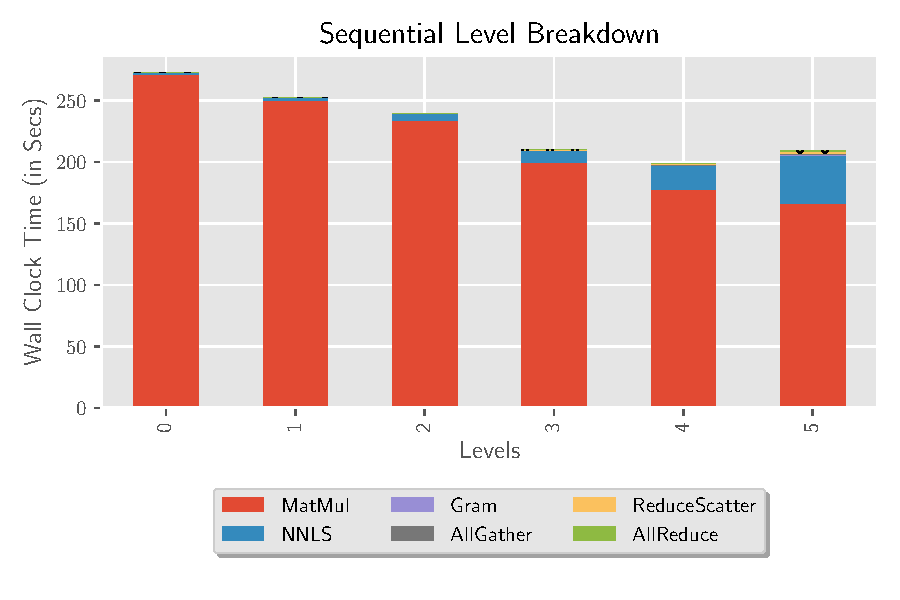
\includegraphics[height=2in, width=\columnwidth]{plots/synthetic_sequential_level_breakdown.pdf}
\caption{Levels Breakdown Timings for 1 Compute Node on Synthetic Data}
\label{fig:seqlevelbreakdown}
\end{center}
\end{figure}

\begin{figure}
\begin{center}
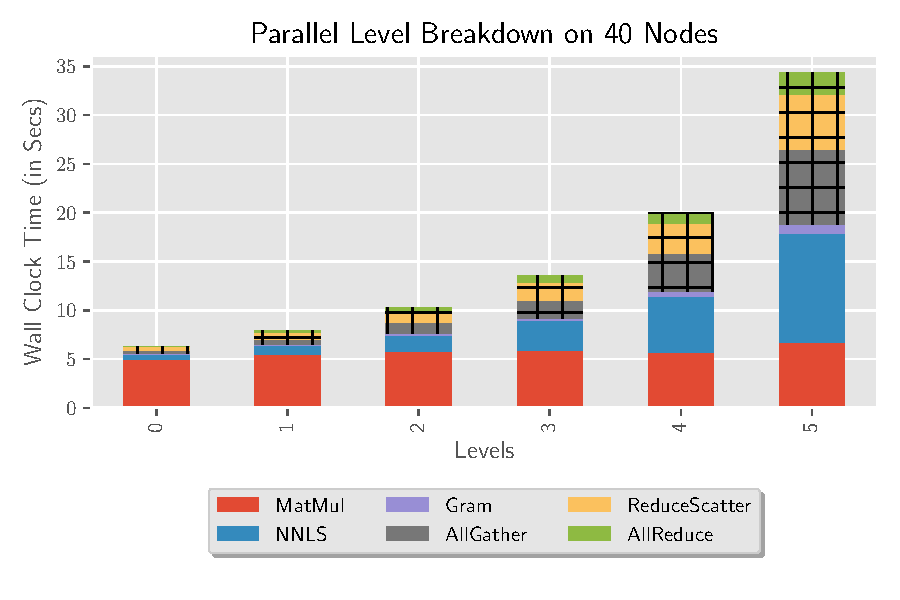
\includegraphics[height=2in, width=\columnwidth]{plots/synthetic_parallel_level_breakdown.pdf}
\caption{Levels Breakdown Timings for 40 Compute Nodes on Synthetic Data}
\label{fig:parallellevelbreakdown}
\end{center}
\end{figure}


%\begin{figure}
%\begin{center}
%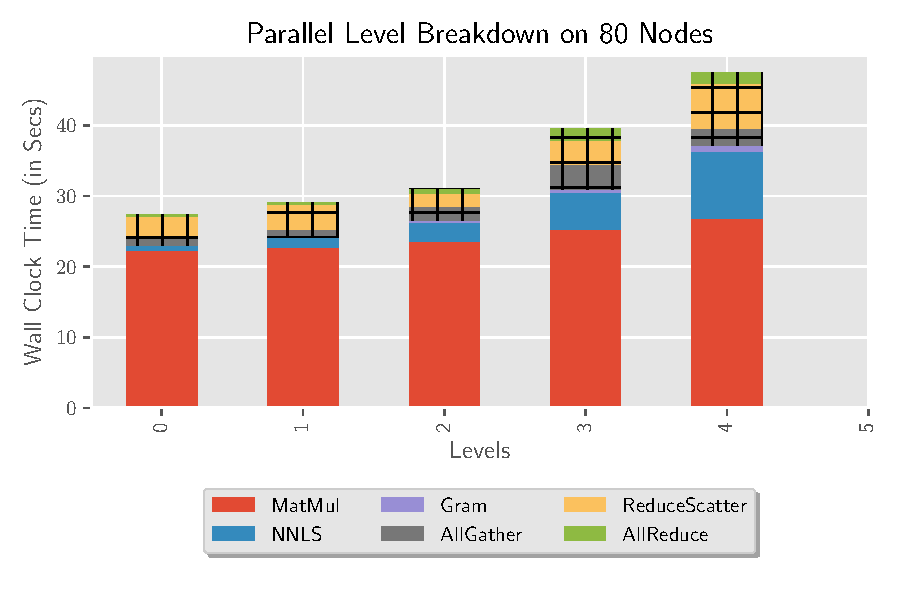
\includegraphics[height=2in, width=\columnwidth]{plots/realworld_parallel_level_breakdown.pdf}
%\caption{Levels Breakdown Timings for 80 Compute Nodes on \image{} Data}
%\label{fig:rwparallellevelbreakdown}
%\end{center}
%\end{figure}


